\documentclass[a4paper,titlepage]{article}
\usepackage[top=1in, bottom=1.25in, left=1.25in, right=1.25in]{geometry}

\parskip=10pt

\usepackage[scaled]{beramono}
\usepackage[T1]{fontenc}

\usepackage{listings}
\lstset{basicstyle=\footnotesize\ttfamily,tabsize=4,breaklines,frame=single}

\usepackage{graphicx}
\usepackage{tikz}

\renewcommand{\figurename}{Gambar}
\renewcommand{\refname}{Referensi}

\begin{document}

	\title{Laporan Tugas I \\ IF2220 Teori Bahasa Formal dan Automata}
	\author{Jonathan Christopher / 13515001 / K-01}
	\maketitle

	\section{Deskripsi Persoalan}

		Persoalan yang harus diselesaikan dalam tugas ini adalah membuat sebuah program yang dapat menerima dan menjalankan sebuah \textit{deterministic finite state automata} (DFA) yang didefinisikan dalam sebuah file terpisah. Program tersebut harus dapat membaca definisi DFA yang terkandung dalam sebuah file eksternal, antara lain daftar \textit{state}, alfabet/daftar simbol masukan, fungsi transisi, serta \textit{state-state} awal dan akhir. Program kemudian akan menerima sebuah \textit{string} input untuk dijalankan pada DFA tersebut. Berdasarkan \textit{string} tersebut, program kemudian harus menampilkan urutan \textit{state-state} yang dilewati, serta apakah \textit{string} tersebut diterima oleh DFA yang sedang dipakai (\textit{state} paling akhir harus merupakan sebuah \textit{final/accepting state}).

		DFA yang harus dibuat didasarkan pada soal 2.2.1 di buku \textit{Introduction to Automata Theory, Languages and Computation}. DFA tersebut merepresentasikan sebuah mesin kelereng yang memiliki beberapa jalur yang dapat dilalui, serta tiga buah tuas yang berubah arah setiap kali setelah dilalui oleh kelereng. Simbol input dari mesin ini adalah slot tempat kelereng dimasukkan, yaitu slot A atau B. Kelereng juga dapat keluar melalui jalur C atau D. Jika kelereng terakhir yang dimasukkan keluar melalui jalur D, maka input diterima; sedangkan bila kelereng terakhir keluar melalui jalur C atau belum ada kelereng yang dimasukkan, input tidak diterima.

		\begin{figure}[h]
		    \centering
		    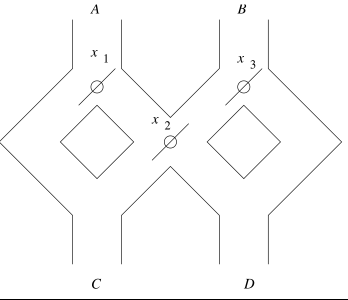
\includegraphics[width=0.5\textwidth]{marble.png}
		    \caption{Mesin kelereng pada \textit{Exercise 2.2.1}}
		    \label{fig:marble}
		\end{figure}

	\section{\textit{Deterministic Finite Automata}}

	\section{Daftar Asumsi}

	\section{\textit{Source Code}}

		\subsection{dfa.h}
			\lstinputlisting[language=C]{../src/dfa.h}

		\subsection{dfa.c}
			\lstinputlisting[language=C]{../src/dfa.c}

		\subsection{main.c}
			\lstinputlisting[language=C]{../src/main.c}

		\subsection{marble.dfa}
			\lstinputlisting{../dfa/marble.dfa}

	\section{Contoh Interaksi dengan Program}

	\begin{thebibliography}{9}

		\bibitem{hopcroft13}
		Hopcroft, John E.; Motwani, Rajeev; Ullman, Jeffrey D.
		(2013).
		\textit{Introduction to Automata Theory, Languages, and Computation (3rd ed.)}
		Pearson.

	\end{thebibliography}

\end{document}